\documentclass[10pt,letterpaper]{article}
\renewcommand{\rmdefault}{ptm}

\usepackage[left=1in,right=1in,top=1in,bottom=1in]{geometry} 
\usepackage{amsmath}
\usepackage{amsfonts}
\usepackage{amsthm}
\usepackage{amssymb}
\usepackage{polynomial}
\usepackage{layouts}

\usepackage{enumerate}

\usepackage{syntax}
\usepackage{gensymb}
\usepackage{cancel}
\usepackage{calc}
\usepackage{enumerate}
\usepackage{xcolor}

\usepackage{minted}

\usepackage[version=0.96]{pgf}
\usepackage{tikz}
\usetikzlibrary{arrows,shapes,automata,backgrounds,petri,positioning}
\usetikzlibrary{decorations.pathmorphing}
\usetikzlibrary{decorations.shapes}
\usetikzlibrary{decorations.text}
\usetikzlibrary{decorations.fractals}
\usetikzlibrary{decorations.footprints}
\usetikzlibrary{shadows}
\usetikzlibrary{calc}
\usetikzlibrary{spy}
\usetikzlibrary{matrix}

\usepackage{tikz-qtree}

\setcounter{tocdepth}{2}
\setcounter{secnumdepth}{4}
\usepackage[bookmarksopen,bookmarksdepth=3]{hyperref}
\usepackage{titlesec}


%define new colors
\definecolor{dark-red}{rgb}{0.8,0.15,0.15}
\definecolor{dark-blue}{rgb}{0.15,0.15,0.7}
\definecolor{medium-blue}{rgb}{0,0,0.5}
\definecolor{dark-green}{rgb}{0.2,0.7,0.7}

%set up color for table of contents
\hypersetup{
    colorlinks, linkcolor={dark-green},
    citecolor={dark-blue}, urlcolor={medium-blue}
}

\usepackage{tocloft}

%preven linebreak between subsection header and its content
\titleformat{\subsection}[runin]{\normalfont\bfseries}{\thesubsection.}{2pt}{}
%\titleformat{\section}[runin]{\normalfont\bfseries\filcenter}{\thesection.}{5pt}{}


\titleformat{\section}[block]
{\normalfont\sffamily\LARGE}
{\thesection}{.2em}{\titlerule\\[.2ex]\bfseries}

%title
\title{\textbf{Math 350 - Advanced Calculus \\ Homework 9}}
\author{Chan Nguyen}

%set numwidth of section
\setlength{\cftsecnumwidth}{1.5cm} 
%make subsection numwidth different than as section
\setlength{\cftsubsecnumwidth}{3cm}
%make subsection indent the same as section
\setlength{\cftsubsecindent}{\cftsecindent} 

\newcommand{\sol}{\textbf{Solution}}

\usepackage{tikz}
\usetikzlibrary{matrix}
\usetikzlibrary{shapes,backgrounds}

\makeatletter
\newcommand{\DESCRIPTION@original@item}{}
\let\DESCRIPTION@original@item\item
\newcommand*{\DESCRIPTION@envir}{DESCRIPTION}
\newlength{\DESCRIPTION@totalleftmargin}
\newlength{\DESCRIPTION@linewidth}
\newcommand{\DESCRIPTION@makelabel}[1]{\llap{#1}}%
\newcommand{\DESCRIPTION@item}[1][]{%
  \setlength{\@totalleftmargin}%
       {\DESCRIPTION@totalleftmargin+\widthof{\textbf{#1 }}-\leftmargin}%
  \setlength{\linewidth}
       {\DESCRIPTION@linewidth-\widthof{\textbf{#1 }}+\leftmargin}%
  \par\parshape \@ne \@totalleftmargin \linewidth
  \DESCRIPTION@original@item[\textbf{#1}]%
}
\newenvironment{DESCRIPTION}
  {\list{}{\setlength{\labelwidth}{0cm}%
           \let\makelabel\DESCRIPTION@makelabel}%
   \setlength{\DESCRIPTION@totalleftmargin}{\@totalleftmargin}%
   \setlength{\DESCRIPTION@linewidth}{\linewidth}%
   \renewcommand{\item}{\ifx\@currenvir\DESCRIPTION@envir
                           \expandafter\DESCRIPTION@item
                        \else
                           \expandafter\DESCRIPTION@original@item
                        \fi}}
  {\endlist}
\makeatother

\allowdisplaybreaks[1]

\begin{document}

\tableofcontents 
\maketitle

\setlength{\parindent}{0pt}
\setlength{\parskip}{1ex}
	\phantomsection
	\subsection*{{\color{purple}\underline{Problem 1}}}
	\addcontentsline{toc}{subsection}{\numberline{}Problem 1}
	Let $f$ be a function that has $n$ derivatives at $a$. The Taylor polynomial of degree $n$
	for $f$ at $a$ is the polynomial $P_{n,a,f}$ in $(x - a)$ given by
	$$P_{n,a,f}(x) = a_0 + a_1(x - a) + a_2(x - a)^2 + \ldots + a_n(x - a)^n$$
	with coefficients $a_k = \dfrac{f^{(k)}(a)}{k!}$.
	\begin{enumerate}[(a)]
	\item Let $f: (0, \infty) \rightarrow \mathbb{R}$ be a function such that $f'(x) = \dfrac{1}{x}$ for all
	$x > 0$ and $f(1) = 0$. Find the Taylor polynomial of degree $n$ for $f$ at $a = 1$.
	\begin{proof}
	We have
	\begin{align*}
		f^{(0)}(x) &= f(x) \\
		f^{(1)}(x) &= \dfrac{1}{x} \\
		f^{(2)}(x) &= \dfrac{-1}{x^2} \\
		f^{(3)}(x) &= \dfrac{-1 \cdot -2}{x^3}\\
		f^{(4)}(x) &= \dfrac{-1 \cdot -2 \cdot -3}{x^4}\\
		f^{(5)}(x) &= \dfrac{-1 \cdot -2 \cdot -3 \cdot -4}{x^5}\\
		\ldots &= \ldots \\
		f^{(k)}(x) &= (-1)^{k+1} \cdot \dfrac{(k - 1)!}{x^{k}}\\
	\end{align*}
	So $$a_k = (-1)^{k+1} \cdot \dfrac{(k-1)!}{a^k}$$
	Thus the Taylor polynomial of degree $n$ for $f$ at $a = 1$ is
	\begin{align*}
	P_{n,a,f} &=& f(1) + 
	(-1)^{1 + 1}\dfrac{(1 - 1)!}{1^1} \cdot (x - 1) + \ldots + 
	(-1)^{n - 1}\dfrac{(n - 1)!}{1^n} \cdot (x - 1)^n \\
	&=& (x - 1) - (x - 1)^2 + 2! \cdot (x - 1)^3 + \ldots + (-1)^{n+1}\dfrac{(n - 1)!}{1^n} \cdot (x - 1)^n\\
	\end{align*}		
	
	\end{proof}
	\item Let $g: \mathbb{R} \rightarrow \mathbb{R}$ be a function such that $g'(x) = \dfrac{1}{\sqrt{1 + x^2}}$
	for all $x > 0$ and $g(0) = 0$. Find the Taylor polynomial of degree $n$ for $g$ at $a = 0$.
	\begin{proof}
	Similarly, 
	\begin{align*}
		g^{(0)}(x) &= g(x) \\
		g^{(1)}(x) &= \dfrac{1}{(1 + x^2)^{1/2}} \\
		g^{(2)}(x) &= \dfrac{-x}{(1 + x^2)^{3/2}} \\
		g^{(3)}(x) &= \dfrac{2x^2 - 1}{(x^2 + 1)^{5/2}} \\
		g^{(4)}(x) &= \dfrac{-6x^3 + 9x}{(x^2 + 1)^{7/2}} \\
		g^{(5)}(x) &= \dfrac{24x^4 - 72x^2 + 9}{(x^2 + 1)^{9/2}} \\
		g^{(6)}(x) &= \dfrac{-120x^5 + 600x^3 - 225x}{(x^2 + 1)^{11/2}} \\
		g^{(7)}(x) &= \dfrac{720x^6 - 5400x^4 + 4050x^2 -225}{(x^2 + 1)^{13/2}} \\
		g^{(8)}(x) &= \dfrac{-5040x^7 + 52920x^5 - 66150x^3 + 11025x}{(x^2 + 1)^{15/2}} \\
		g^{(9)}(x) &= \dfrac{40320x^8 - 564480x^5 - 1058400x^3 + 352800x^2 + 11025}{(x^2 + 1)^{17/2}} \\
	\end{align*}	
	It seems like the general for the $n$th derivative of $\dfrac{1}{\sqrt{1 + x^2}}$ is a little
	overkill. Note that we only need to find the $n$th derivative at $a = 0$, i.e. $g^{(k)}(0)$, but if 
	we look at the pattern of the first 9 derivatives, we see that every even term is actually zeroed out.	
	\begin{align*}
		g^{(0)}(0) &= 0 \\
		g^{(1)}(0) &= \dfrac{1}{(1 + x^2)^{1/2}} = 1\\
		g^{(2)}(0) &= 0 \\
		g^{(3)}(0) &= \dfrac{2x^2 - 1}{(x^2 + 1)^{5/2}} = -1\\
		g^{(4)}(0) &= 0 \\
		g^{(5)}(0) &= \dfrac{24x^4 - 72x^2 + 9}{(x^2 + 1)^{9/2}} = 9 \\
		g^{(6)}(0) &= 0 \\
		g^{(7)}(0) &= \dfrac{720x^6 - 5400x^4 + 4050x^2 -225}{(x^2 + 1)^{13/2}} = -225\\
		g^{(8)}(0) &= 0 \\
		g^{(9)}(x) &= \dfrac{40320x^8 - 564480x^5 - 1058400x^3 + 352800x^2 + 11025}{(x^2 + 1)^{17/2}} = 11025 \\
	\end{align*}
	Now the remain task is to find out what is the general pattern of the sequence $1, 1, 225, 11025$ since the 
	alternating sign can be handle easily by adding $(-1)^n$. By factoring out each of this number, we see that
	\begin{align*}
		1     &= 1 \\
		1     &= 1 \\
		9     &= 3^2 \\
		225   &= 3^2 \cdot 5^2 \\
		11025 &= 3^2 \cdot 5^2 \cdot 7^2 \\
	\end{align*}
	which is the product of odd square, so we have
	\begin{align*}
		\bigg[\displaystyle\prod_{i=1}^{n}(2i - 1)\bigg]^2
	\end{align*}
	To find a more compact formula for this expression, we complete the factorial by write it as
	\begin{align*}
		\displaystyle\prod_{i=1}^{n}(2i - 1)
		&= \dfrac{1 \cdot 2 \cdot 3 \cdot 4 \cdot 5 \cdot 6 \cdots (2n - 1) \cdot 2n}{2 \cdot 4 \cdot 6 \cdots 2n} \\
		&= \dfrac{(2n)!}{2^n(1 \cdot 2 \cdot 3 \cdots n)} \\
		&= \dfrac{(2n)!}{2^nn!} \\
	\end{align*}
	Now try out some values for $k$, we have $k = 7$, yields $225$ which is
	$$\bigg[\dfrac{(2 \cdot 3)!}{3! \cdot 2^3}\bigg]^2
	= \bigg[\dfrac{(7 - 1)!}{((7 - 1)/2)! \cdot 2^{(7 - 1)/2}}\bigg]^2$$
	Generally,
	$$g^{(k)}(0) = (-1)^{\lfloor \frac{k}{2} \rfloor}\dfrac{(k - 1)!}{[(k - 1)/2]! \cdot 2^{\frac{k - 1}{2}}}$$	
	So the Taylor polynomial of degree $n$ for $g$ at $a = 0$ is
$$
P_{n,0,g}= 
\dfrac{1}{1!} \cdot x +
\dfrac{-1}{3!} \cdot x^3 +
\dfrac{9}{5!} \cdot x^5 +
\dfrac{-225}{7!} \cdot x^7 + 
\ldots + 
\dfrac{(-1)^{\lfloor \frac{n}{2} \rfloor}\dfrac{(n - 1)!}{[(n - 1)/2]! \cdot 2^{\frac{n - 1}{2}}}}{n!} \cdot x^n
$$
	
	
	
	\end{proof}
	
	\end{enumerate}
	
	
	\phantomsection
	\subsection*{{\color{purple}\underline{Problem 2}}}
	\addcontentsline{toc}{subsection}{\numberline{}Problem 2}
	Let $f$ have $n$ derivatives at $a$. Prove that
	$$\displaystyle\lim_{x\to a} \dfrac{f(x) - P_{n,f,a}(x)}{(x - a)^n} = 0$$
	\begin{proof}
		Recall 
		$$P_{n,a,f}(x) = a_0 + a_1(x - a) + a_2(x - a)^2 + \ldots + a_n(x - a)^n$$
		with coefficients $a_k = \dfrac{f^{(k)}(a)}{k!}$. \\
		
		Let $g(x) = P_{n,a,f}(x)$, we notice that
	\begin{align*}
		g^{(1)}(a) &= 1! \cdot a_1  \\
		g^{(2)}(a) &= 2! \cdot a_2 \\
	    \ldots &= \ldots \\
	    g^{(k)}(a) &= k! \cdot a_k 
	\end{align*}
	Hence, $g^{(k)}(a) = k! \cdot \dfrac{f^{(k)}(a)}{k!} = f^{(k)}(a)$. Then
	\begin{align*}
	\displaystyle\lim_{x\to a}[f^{(k)}(x) - g^{(k)}(x)] &= 0 
	\end{align*}
	for all $0 \leq k \leq n$. \\
	
	\textbf{...not done!} 
	\end{proof}
	
	\phantomsection
	\subsection*{{\color{purple}\underline{Problem 3}}}
	\addcontentsline{toc}{subsection}{\numberline{}Problem 3}
	Two functions $f$ and $g$ are equal up to order $n$ at $a$ if 
	$$\displaystyle\lim_{x\to a}\dfrac{f(x) - g(x)}{(x - a)^n} = 0$$
	\begin{enumerate}[(a)]
		\item Let $P(x) = p_0 + p_1(x - a) + p_2(x - a)^2 + \ldots + p_M(x - a)^M$ and
		$Q(x) = q_0 + q_1(x - a) + \ldots q_N(x - a)^N$ be two polynomials in $(x - a)$ of degrees $M, N \leq n$.
		Prove that if $P$ and $Q$ are up to order $n$ at $a$ then $P = Q$.
		\begin{proof}
		Without loss of generality, assume that $N \leq M$. Since $P$ and $Q$ are up to order $n$ at $a$, we have that
	\begin{align*}
		\displaystyle\lim_{x\to a}\dfrac{P(x) - Q(x)}{(x - a)^n} &=& 0
	\end{align*}
	Consider 
	$$P(x) - Q(x) = (p_0 - q_0) + (p_1 - q_1)(x - a) + (p_2 - q_2)(x - a)^2 + \ldots + (p_N - q_N)(x - a)^N + \ldots p_M(x - a)^M$$
	What we want to show is that $P(x) - Q(x) = 0 \Rightarrow P(x) = Q(x)$. On the other hand,
	we claim that 
	\begin{eqnarray}
	\displaystyle\lim_{x\to a}\dfrac{f(x) - g(x)}{(x - a)^n} \Rightarrow \displaystyle\lim_{x\to a}\dfrac{f(x) - g(x)}{(x - a)^k}, 0 \leq k \leq n
	\end{eqnarray}		
		
		Let $h(x) = f(x) - g(x)$, since $\displaystyle\lim_{x\to a}\dfrac{h(x)}{(x - a)^k} = 0$, by definition of limit, given 
		$\epsilon > 0$ , there exists $\delta > 0$ such that if $|x - a| < \delta$ then $\bigg|\dfrac{h(x)}{(x - a)^n} - 0\bigg| < \epsilon$. So we can choose
	$\gamma = \min(\delta, 1)$, then if $|x - a| < \gamma$ then, 		
		$$\bigg|\dfrac{h(x)}{(x - a)^n} \cdot (x - a)^{m} - 0 \bigg| =
		\bigg|\dfrac{h(x)}{(x - a)^n}\bigg| \cdot  |x - a|^{m} < \epsilon \cdot 1 = \epsilon$$
		where $m = n - k$.		
		So (1) holds for any $k, 0 \leq k \leq n$.
		Inductively choose $k = 0, 1, \ldots n$, we have
		\begin{itemize}
			\item $k = 0$:\\
			$\displaystyle\lim_{x\to a} (p_0 - q_0) + (p_1 - q_1)(x - a) + (p_2 - q_2)(x - a)^2 + \ldots + (p_N - q_N)(x - a)^N + \ldots p_M(x - a)^M = 0$
			$$\Rightarrow p_0 - q_0 = 0 \Rightarrow p_0 = q_0$$
			\item $k = 1$:\\
			$\displaystyle\lim_{x\to a} (p_1 - q_1) + (p_2 - q_2)(x - a) + \ldots + (p_N - q_N)(x - a)^{N-1} + \ldots p_M(x - a)^{M - 1} = 0$
			$$\Rightarrow p_1 - q_1 = 0 \Rightarrow p_1 = q_1$$
			\item $k = \ldots$
			\item $k = n$
			$\displaystyle\lim_{x\to a} p_n{(x - a)^n} = 0$ 
			$$\Rightarrow p_n = 0$$
		\end{itemize}
		Thus it must he case that $M = N$ and $p_k - q_k = 0$ for all $0 \leq k \leq N = n$, in other words $P(x) = Q(x)$.		
		
	\end{proof}
		
		\item Let $f$ be $n$ times differentiable at $a$ and suppose that $P$ is a polynomial $(x - a)$
		of degree $\leq n$ that equals $f$ up to order $n$ at $a$. Prove that
		$P = P_{n,f,a}$, the Taylor polynomial of degree $n$ for $f$ at $a$.
		\begin{proof}
			We have
			$$P_{n,a,f}(x) = a_0 + a_1(x - a) + a_2(x - a)^2 + \ldots + a_n(x - a)^n  \text{ with } a_k = \dfrac{f^{(k)}(a)}{k!}$$
			and
			$$P_{n,a}(x) = a'_0 + a'_1(x - a) + a'_2(x - a)^2 + \ldots a'_n(x - a)^n$$
			Using the same technique from part (a), we have
			\begin{align*}
			a_0 &= a'_0 \\
			a_1 &= a'_1 \\
			a_2 &= a'_2 \\
			\ldots &= \ldots \\
			a_n &= a'_n \\
			\end{align*}
			It follows that $P_{n,a} = P_{n,f,a}$. This is actually the result of part (a) since $P_{n,f,a}$ and $P_{n,a}$ are the same as
			$P, Q$.
		\end{proof}
	\end{enumerate}
	
	\phantomsection
	\subsection*{{\color{purple}\underline{Problem 4}}}
	\addcontentsline{toc}{subsection}{\numberline{}Problem 4}
	Let $f: \mathbb{R} \rightarrow \mathbb{R}$ be a function such that $f'(x) = f(x)$ for all $x$
	and $f(0) = 1$. Prove that, for all $n$ and all $x$, 
	$$|f(x) - P_{n,0,f}(x)| \leq \dfrac{F_x|x|^{n+1}}{(n + 1)!}$$
	where $F_x = \sup\{|f(y)| : |y| \leq |x|\}$.
	\begin{proof}
	First we will show that the two conditions $f'(x) = f(x)$ for all $x$ and $f(0) = 1$ implies that
	$f(x) = e^x$. The second part is just the result of the remainder term of Taylor polynomial of $e^x$.
	First note that $f'(x) = f(x)$ implies $f^{(k)}$ exists and $f^{(k)} = f(x)$ because $f''(x) = (f'(x))' = f'(x)$ and so on.
	Write $f(x)$ in Taylor polynomial form $P_{n,f,a}$,
	\begin{align*}
	P_{n,f,a} 
&= f(0) + \dfrac{f(a)}{1!}(x - a) + \dfrac{f(a)}{2!}(x - a)^2 + \ldots + \dfrac{f(a)}{n!}(x - a)^n \\ 
&= 1 + \dfrac{f(a)}{1!}(x - a) + \dfrac{f(a)}{2!}(x - a)^2 + \ldots + \dfrac{f(a)}{n!}(x - a)^n 
	\end{align*}	 
	At $a = 0$, we have
		$$P_{n,f,0} = 1 + x + \dfrac{x^2}{2!} + \ldots + \dfrac{x^n}{n!} $$ 
	
	On the other hand, we know that from lecture notes:
	$$e^x = 1 + x + \dfrac{x^2}{2!} + \ldots + \dfrac{x^n}{n!} + R_{n,x} = 1 + x + \dfrac{x^2}{2!} + \ldots + \dfrac{x^n}{n!} + \dfrac{f^{n+1}(c)}{(n + 1)!} \cdot x^{n+1}$$
	Then
	$$f(x) - P_{n,f,0} = e^x - P_{n,f,0} = R_{n,x} = \dfrac{f^{n+1}(c)}{(n + 1)!} \cdot x^{n+1} = \dfrac{f(c)}{(n + 1)!} x^{n+1}$$
	for some $c$ between $x$ and $0$. \\
	Moreover, since  $F_x = \sup\{|f(y)| : |y| \leq |x|\}$, by definition of supremum, $F_x \leq f(c)$ for all $c$ between $x$ and $0$. Thus
	$$|f(x) - P_{n,f,0}| = |R_{n,x}| = \bigg|\dfrac{f(c)}{(n + 1)!} x^{n+1}\bigg| \leq \dfrac{F_x|x|^{n+1}}{(n + 1)!}$$
	\end{proof}
	
	\phantomsection
	\subsection*{{\color{purple}\underline{Problem 5}}}
	\addcontentsline{toc}{subsection}{\numberline{}Problem 5}
	Given a function $f$ and two integers $M \geq 0$ and $N \geq 0$, the Pade approximant of order $[M/N]$
	of $f$ (at $0$) is the rational function
	$$R(x) = \dfrac{a_0 + a_1x + a_2x^2 + \ldots + a_Mx^M}{
	1 + b_1x + b_2x^2 + \ldots + b_Nx^N}$$
	that agrees with $f(x)$ to the highest possible order which amounts to 
	\begin{align*}
		R(0)   &= f(0) \\
		R'(0)  &= f'(0) \\
		R''(0) &= f''(0) \\
		\ldots &= \ldots \\
		R^{(M + N)}(0) &= f^{(M + N)}(0)	
	\end{align*}
	Let $f: \mathbb{R} \rightarrow \mathbb{R}$ be such that $f'(x) = f(x)$ for all $x$ and $f(0) = 1$.
	Find the Pade approximant of order $[2/2]$ for $f$. 
	\begin{proof}
	The Pade approximant of order $[2/2]$ is given by
	$$R(x) = \dfrac{a_0 + a_1x + a_2x^2}{1 + b_1x + b_2x^2}$$
	For $M = 2, N = 2$, we want to satisfy
	$$
	 \dfrac{a_0 + a_1x + a_2x^2}{1 + b_1x + b_2x^2} = 
	 c_0 + c_1x + c_2x^2 + c_3x^3 + c_4x^4$$
	 
	where 
	$$f(x) = e^x = 
	1 + x + \dfrac{x^2}{2!} + \dfrac{x^3}{3!} + \dfrac{x^4}{4!}$$
 	Multiplying up the denominator and then equating coefficients up to $x^4$, we have that
\begin{align*} 
 a_0 + a_1x + a_2x^2 
&=& (1 + b_1x + b_2x^2) \cdot (c_0 + c_1x + c_2x^2 + c_3x^3 + c_4x^4) \\
&=& c_0 + c_1x + c_2x^2 + c_3x^3 + c_4x^4 + \\
& & b_1c_0x + b_1c_1x^2 + b_1c_2x^3 + b_1c_3x^4 + b_1c_4x^5 + \\
& & b_2c_0x^2 + b_2c_1x^3 + b_2c_2x^4 + b_2c_3x^5 + b_2c_4x^6
\end{align*}
	which yields a system of equations
 	\begin{align*}
		a_0 &= c_0 = 1 \\ 	
		a_1 &= c_1 + b_1c_0 \\
		a_2 &= c_2 + c_1b_1 + c_0b_2\\
		0   &= c_3 + b_1c_2 + b_2c_1 \\
		0   &= c_4 + b_1c_3 + b_2c_2  \\
 	\end{align*}
 	where 
 		$c_0 = 1 , \,\,\,\, c_1 = 1 , \,\,\,\, c_2 = \dfrac{1}{2}
 		, \,\,\,\, c_3 = \dfrac{1}{6}, \,\,\,\, c_4 = \dfrac{1}{24} $.
 	Solving this system of equations we have 
 	\begin{align*}
 		&  a_0 = 1, a_1 = \dfrac{1}{2}, a_2 = \dfrac{1}{12} \\
 		&  b_0 = 1, b_1 = \dfrac{-1}{2}, b_2 = \dfrac{1}{12} 
 	\end{align*}
	Therefore, the Pade approximant of order $[2/2]$ is
	$$
	\dfrac{1 + \dfrac{x}{2} + \dfrac{x^2}{12}}{1 - \dfrac{x}{2} + \dfrac{x^2}{12}} = 
	\dfrac{12 + 6x + x^2}{12 - 6x + x^2}
	$$
	\end{proof}
	
	\phantomsection
	\subsection*{{\color{purple}\underline{Problem 6}}}
	\addcontentsline{toc}{subsection}{\numberline{}Problem 6}
	Let $f$ and $g$ be integrable on $[a, b]$ and let $c$ be a constant.
	\begin{enumerate}[(a)]
		\item Prove that $c \cdot f$ is integrable on $[a, b]$ on 
		$\displaystyle\int_{a}^{b} c \dot f = c \cdot \displaystyle\int_{a}^{b} f$.
		\begin{proof}
		Since $f$ is integrable on $[a, b]$, for every $\epsilon > 0$, there exists
		a partition $P$ in $[a, b]$ such that
		$$U(f, P) - L(f, P) < \epsilon$$
		Let 
		\begin{align*}
 			m_i  &= \inf\{f(x) : t_{i-1} \leq x \leq t_i\} \\
			M_i  &= \sup\{f(x) : t_{i-1} \leq x \leq t_i\} \\
			m'_i &= \inf\{c \cdot f(x) : t_{i-1} \leq x \leq t_i\} \\
			M'_i &= \sup\{c \cdot f(x) : t_{i-1} \leq x \leq t_i\} \\
		\end{align*}
		Since $c > 0$ is just a constant, we have $m'_i = c \cdot m_i$ and $M'_i = c \cdot M_i$. Let
		Choose $\epsilon = \dfrac{\epsilon}{c}$ for $P$, we have
	\begin{align*}
		U(cf, P) - L(cf, P) = c[U(f, P) - L(f, P)] < \dfrac{\epsilon}{c} \cdot c = \epsilon
	\end{align*}
		
		\end{proof}
		
		\item Prove that $f + g$ is integrable on $[a, b]$ and 
		$\displaystyle\int_{a}^{b} (f + g) = \displaystyle\int_{a}^{b} f + 
		\displaystyle\int_{a}^{b} g$.
		\begin{proof}
		Let 
		\begin{align*}
 			m_i &= \inf\{f(x) : t_{i-1} \leq x \leq t_i\} \\
			M_i &= \sup\{f(x) : t_{i-1} \leq x \leq t_i\} \\
			n_i &= \inf\{g(x) : t_{i-1} \leq x \leq t_i\} \\
			N_i &= \sup\{g(x) : t_{i-1} \leq x \leq t_i\} \\
			s_i &= \inf\{(f + g)(x) : t_{i-1} \leq x \leq t_i\} \\
			S_i &= \sup\{(f + g)(x) : t_{i-1} \leq x \leq t_i\} \\
		\end{align*}
		We claim that $m_i + n_i \leq s_i$ since $m_i \leq f(x)$ and $n_i \leq g(x)$ for all $x \in [t_{i-1}, t_i]$, so 
		$m_i + n_i \leq f(x) + g(x)$ which implies $m_i + n_i$ is a lower bound of $f(x) + g(x) = (f + g)(x)$, where
		$s_i$ is the greatest as such, thus $m_i + n_i \leq s_i$. \\
		Similarly, we also claim that $M_i + N_i \geq S_i$ since $M_i \geq f(x)$ and $N_i \geq g(x)$ for all $x \in [t_{i-1}, t_i]$
		so $M_i + N_i \geq (f + g)(x)$ which implies $M_i + N_i$ is an upper bound of $(f + g)(x)$, where $S_i$ is the least 
		as such, thus $M_i + N_i \geq S_i$. \\
		Thus, 
		$$U(f + g, P) \leq U(f, P) + U(g, P)$$
		$$L(f + g, P) \geq L(f, P) + L(g, P)$$
		On the other hand, since $f, g$ are both integrable on $[a, b]$, for all $\epsilon > 0$, there exists $P_1, P_2$, such that
		$$U(f, P_1) - L(f, P_1) < \dfrac{\epsilon}{2}$$
		$$U(g, P_2) - U(g, P_2) < \dfrac{\epsilon}{2}$$
		Let $P = P_1 \cup P_2$, so that $P$ contains both $P_1, P_2$ then by Lemma, we have
		$$L(f, P_1) \leq L(f, P) \text{ and } L(f, P_2) \leq L(f, P)$$
		$$U(f, P_1) \geq L(f, P) \text{ and } U(f, P_2) \geq U(f, P)$$ 
		Hence,
		$$U(f + g, P) - U(f + g, P) < U(f, P) - L(f, P) + U(f, P) - L(f, P) < \dfrac{\epsilon}{2} + \dfrac{\epsilon}{2} = \epsilon$$
		\end{proof}
	\end{enumerate}
	
	\phantomsection
	\subsection*{{\color{purple}\underline{Problem 7}}}
	\addcontentsline{toc}{subsection}{\numberline{}Problem 7}
	Prove that if $f$ is integrable on $[a, b]$, then $|f|$ is integrable on $[a, b]$ and 
	$\displaystyle\bigg|\int_{a}^{b} f \bigg| \leq \displaystyle\int_{a}^{b} |f|$
	\begin{proof}
	By definition of absolute, we have
	$$
		-|f| \leq f \leq |f|
	$$
	On the other hand, 
	$$L(f, P) \leq f \leq U(f, P)$$
	where
	\begin{align*}
		L(f, P) &= \displaystyle\sum_{i=1}^{n} m_i(t_{i} - t_{i-1}) \\
		U(f, P) &= \displaystyle\sum_{i=1}^{n} M_i(t_{i} - t_{i-1}) 
	\end{align*}
	Since $t_i - t_{i-1}$ is the length of a subinterval, $t_i - t_{i-1} \geq 0$, so the $L(f, P)$ and $U(f, P)$ depend
	only on $m_i$ and $M_i$, where
	\begin{align*}
		m_i &= \inf\{f(x): t_{i-1} \leq x \leq t_{i} \} \\
		M_i &= \sup\{f(x): t_{i-1} \leq x \leq t_{i} \} 	
	\end{align*}
	Let 
	\begin{align*}
		m'_i &= \inf\{|f|(x): t_{i-1} \leq x \leq t_{i} \} \\
		M'_i &= \sup\{|f|(x): t_{i-1} \leq x \leq t_{i} \} 	
	\end{align*}
	It's easy to see that
	$M_i \leq M'_i$
	and $m_i \leq m'_i$. Thus
	$$-\displaystyle\int_{a}^{b} |f| \leq \displaystyle\int_{a}^{b} f \leq \displaystyle\int_{a}^{b} |f|$$
	or 
	$$\displaystyle\bigg|\int_{a}^{b} f \bigg| \leq \displaystyle\int_{a}^{b} |f|$$
	\end{proof}
	
	\phantomsection
	\subsection*{{\color{purple}\underline{Problem 8}}}
	\addcontentsline{toc}{subsection}{\numberline{}Problem 8}
	Evaluate without doing any computations
	\begin{enumerate}[(a)]
		\item $\displaystyle\int_{-1}^{1} x^3 \sqrt{1 - x^2} dx$
		\begin{proof}
	\begin{align*}
		\displaystyle\int_{-1}^{1} x^3 \sqrt{1 - x^2} 
		&= \displaystyle\int_{-1}^{0} x^3 \sqrt{1 - x^2} + \displaystyle\int_{0}^{1} x^3 \sqrt{1 - x^2} \\
		&= -\displaystyle\int_{0}^{1} x^3 \sqrt{1 - x^2} + \displaystyle\int_{0}^{1} x^3 \sqrt{1 - x^2} = 0
	\end{align*}
		\end{proof}
		
		\item $\displaystyle\int_{-1}^{1} (x^5  + 1)\sqrt{1 - x^2} dx$
		\begin{proof}
		\begin{align*}
		\displaystyle\int_{-1}^{1} (x^5  + 1)\sqrt{1 - x^2} 
		&= \displaystyle\int_{-1}^{0} (x^5  + 1)\sqrt{1 - x^2} + \displaystyle\int_{0}^{1} (x^5  + 1)\sqrt{1 - x^2} \\
		&= -\displaystyle\int_{0}^{1} (x^5  + 1)\sqrt{1 - x^2} + \displaystyle\int_{0}^{1} (x^5  + 1)\sqrt{1 - x^2} = 0
		\end{align*}
		\end{proof}
	\end{enumerate}
	
	
	\phantomsection
	\subsection*{{\color{purple}\underline{Problem 9}}}
	\addcontentsline{toc}{subsection}{\numberline{}Problem 9}
	Prove that if $f(x) = x^3$, then $\displaystyle\int_{a}^{b} f = \dfrac{b^4 - a^4}{4}$, by considering
	upper and lower sums for partitions $[a, b]$ into $n$ equal subintervals, using the formula:
	$1^3 + 2^3 + \ldots + n^3 = (1 + 2 + \ldots + n)^2$ for the sum of the cubes of the first $n$
	positive integers.
	\begin{proof}
	We have
	$$\displaystyle\int_{a}^{b} x^3 = \displaystyle\int_{0}^{b} x^3 - \displaystyle\int_{0}^{a} x^3$$
	Consider a partition $P$ in $[0, a]$, and divide this partition into $n$ equal subintervals of length
	$\dfrac{a}{n}$. So we have
	\begin{align*}
		t_0 &= 0 \\
		t_1 &= \dfrac{a}{n} \\
		t_2 &= a + \dfrac{2a}{n} \\
		t_3 &= a + \dfrac{3a}{n} \\
	    \ldots &=  \ldots \\
		t_i &= a + \dfrac{ia}{n}
	\end{align*}
	Let 
	\begin{align*}
		m_i &= \inf\{x^3 : x \in [t_{i-1}, t_i]\} \\
		M_i &= \sup\{x^3 : x \in [t_{i-1}, t_i]\} \\
	\end{align*}
	For any subinterval $[t_{i-1}, t_i]$, we have $m_i = t_{i-1}^3$ and $M_i = t_i^3$ because $t_{i-1} < t_{i}$ and $x^3$ is
	increasing ($f'(x) = 3x^2 \geq 0, \forall x$). Thus
	\begin{align*}
		M(f, P) 
		 &= \displaystyle\sum_{i=1}^{n} M_i(t_{i} - t_{i-1}) \\
		 &= \displaystyle\sum_{i=1}^{n} \bigg[\dfrac{ia}{n} \bigg]^3 \cdot \dfrac{a}{n} \\	
		 &= \dfrac{a^4}{n^4} \displaystyle\sum_{i=1}^{n} i^3 \\ 
		 &= \dfrac{a^4}{n^4} \cdot \bigg[\dfrac{n(n + 1)}{2}\bigg]^2 \\
		 &= \dfrac{a^4}{4} \cdot \dfrac{n^4 + 2n^3 + n^2}{n^4} \\ 
	\end{align*}	
	Since $\displaystyle\lim_{n\to \infty} \dfrac{n^4 + 2n^3 + n^2}{n^4} = 1$, for sufficiently large $n$, we have
	$$M(f, P) = \dfrac{a^4}{n^4}$$
	Similarly, for the lower bound
	\begin{align*}
	L(f, P) 
	     &= \displaystyle\sum_{i=1}^{n} m_i(t_{i} - t_{i-1}) \\
		 &= \displaystyle\sum_{i=1}^{n} \bigg[\dfrac{(i - 1)a}{n} \bigg]^3 \cdot \dfrac{a}{n} \\
		 &= \displaystyle\sum_{i=0}^{n-1} \bigg[\dfrac{(i - 1)a}{n} \bigg]^3 \cdot \dfrac{a}{n} \\		
		 &= \dfrac{a^4}{n^4} \displaystyle\sum_{i=0}^{n-1} i^3 \\ 
		 &= \dfrac{a^4}{n^4} \cdot \bigg[\dfrac{(n - 1)n}{2}\bigg]^2 \\
		 &= \dfrac{a^4}{n^4} \cdot \dfrac{n^4 - 2n^3 + n^2}{4} \\
		 &= \dfrac{a^4}{4} \cdot \dfrac{n^4 - 2n^3 + n^2}{n^4} \\ 
	\end{align*}	
	Again, we have that $\displaystyle\lim_{n\to \infty}\dfrac{n^4 - 2n^3 + n^2}{n^4} = 1$, so for sufficiently large $n$, 
	we have $L(f, P) = \dfrac{a^4}{n^4}$. Hence,
	$$\dfrac{a^4}{4} \leq \displaystyle\int_{0}^{a} f \leq \dfrac{a^4}{4}$$
	which implies $\displaystyle\int_{0}^{a} f = \dfrac{a^4}{4}$. 
	Similarly, we have
	$\displaystyle\int_{0}^{b} f = \dfrac{b^4}{4}$.
	It follows that,
	$$\displaystyle\int_{a}^{b} x^3 = \displaystyle\int_{0}^{b} x^3 - \displaystyle\int_{0}^{a} x^3 =
	 \dfrac{b^4}{4} - \dfrac{a^4}{4} = \dfrac{b^4 - a^4}{4} $$
	
	\end{proof}
	
	\phantomsection
	\subsection*{{\color{purple}\underline{Problem 10}}}
	\addcontentsline{toc}{subsection}{\numberline{}Problem 10}
	Decide which of the following functions are integrable on $[0, 2]$ and calculate the integral
	sum if you can.
	\begin{enumerate}[(a)]
		\item 
		$f(x) = 
		\begin{cases}
			x + [x] &, x \text{ rational } \\
			0 &, x \text{ irrational } 
		\end{cases}
		$
		\begin{proof}
		We claim that $f(x)$ is not integrable, in order to prove this fact, for all partition $P$ of $[0, 2]$ such that
		given $\epsilon > 0$, then $U(f,P) - L(f, P) > \epsilon$. \\
		Let $P = \{t_0, t_1, \ldots, t_n\}$ be any partition of $[0, 2]$, then we have at least one point $t_i \geq 1$
		which implies there is some $M_i = \sup\{f(x): t_{i-1} \leq x \leq t_i\} \geq 1$ because $[x]$ is the integer
		part that is less than equal to $x$, plus $x$ in $[0, 2]$, so it must be $\geq 1$ for some interval $[t_i, t_j]$ if 
		$x$ is rational. Hence, $U(f, P) \geq 1$ because 
		$$U(f, P) = \displaystyle\sum_{i=1}^{n} M_i(t_i - t_{i-1})$$ 
		where $M_i \geq 0$, and there some $i$ such that $M_i \geq 1$. \\
		On the other hand, $L(f, P)$ is always $0$ because $x \in [0, 2]$ and $f(x) = x + [x]$. Thus
		$$U(f, P) - L(f, P) \geq 1 \text{ for all } P \text{ of } [0, 2]$$
		Any $\epsilon > 1$ would suffice.
		\end{proof}
		
		\item $f$ is the function shown in Figure 1 (set $f(0) = 0$).
		\begin{center}
			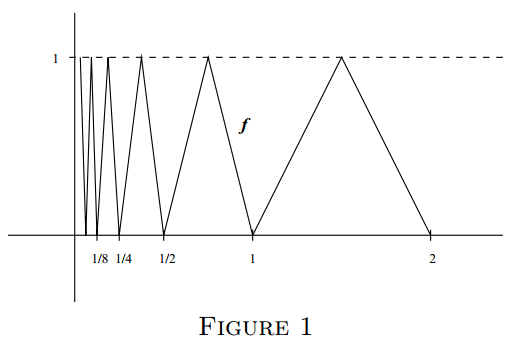
\includegraphics[scale=0.5]{hw9.png}
		\end{center}
		\begin{proof}
		First we note that
		\begin{itemize}
			\item $f$ is bounded above by $1$ in $[0, 2]$.
			\item $f$ is discontinuous at $x = 0$.
		\end{itemize}
		As we can see each area of the triangle can be computed by height $h = 1$, a
		and base
		\begin{align*}
			b_0 &= 2 - 1 \\
			b_1 &= 1 - \dfrac{1}{2} \\
			b_2 &= \dfrac{1}{2} - \dfrac{1}{4} \\
			\ldots &= \ldots \\
			b_3 &= \dfrac{1}{2^{n}} - \dfrac{1}{2^{n+1}} \\
			\ldots &= \ldots
		\end{align*}
		
		So total area of all triangles is
\begin{align*}
	A 
	&= \dfrac{1}{2} \cdot 1 \cdot (2 - 1) + \displaystyle\sum_{i=0}^{\infty} \dfrac{1}{2} b_i \cdot h_i \\
	&=  \dfrac{1}{2} + \displaystyle\sum_{i=0}^{\infty} \bigg(\dfrac{1}{2^{i}} - \dfrac{1}{2^{i+1}} \bigg)\\
	&=  \dfrac{1}{2} + \displaystyle\sum_{i=0}^{\infty} \dfrac{2 - 1}{2^{i+1}}\\ 
	&=  \dfrac{1}{2} + \displaystyle\sum_{i=1}^{\infty} \bigg(\dfrac{1}{2}\bigg)^i\\ 
	&=  \dfrac{1}{2} + \bigg(\dfrac{1}{2} + \dfrac{1}{4} + \dfrac{1}{8} + \ldots \bigg)\\
	&=  \dfrac{1}{2} \cdot \bigg(1 + \dfrac{1}{2} + \dfrac{1}{4} + \ldots \bigg)\\ 
\end{align*}		
	Recall the Geometric sum for $\dfrac{1}{2} < 1$, we have
	$$\displaystyle\sum_{i=0}^{\infty} \bigg(\dfrac{1}{2}\bigg)^i = \dfrac{1}{1 - \dfrac{1}{2}}
	= \dfrac{1}{1/2} = 2$$
	Thus the area is $\dfrac{1}{2} \cdot 2 = 1$. \\
	To prove that $f$ is integrable formally, we have to consider an $\epsilon > 0$. Notice 
	that, although $f$ is not continuous at $0$, it's in fact continuous at $[\epsilon, 2]$ 
	for $0 < \epsilon < 2$.
	But continuity implies that $f$ is integrable, so let $P_i$ be the partition of 
	of the $i$ triangle in the picture, i.e.
	\begin{align*}
		P_1 &= \{2, 1\} \\
		P_2 &= \{1, \dfrac{1}{2}\} \\
		P_3 &= \{\dfrac{1}{2}, \dfrac{1}{4}\} \\
		\ldots &= \ldots \\
		P_n &= \{\dfrac{1}{2^{n}}, \dfrac{1}{2^{n+1}}\} \\
		\ldots &= \ldots
	\end{align*}
	For each of these intervals, we have 
	$$U(f, P_i) - L(f, P_i) < \dfrac{\epsilon}{2^i}$$
	Now we choose $P = \displaystyle\bigcup_{i=1}^{\infty} P_i$, then
	\begin{align*}
	U(f, P) - L(f, P) &=\displaystyle\sum_{i=0}^{n} U(f, P_i) - L(f, P_i) \\
	&< \displaystyle\sum_{i=1}^{n} \dfrac{\epsilon}{2^i} 
	= \epsilon \cdot \displaystyle\sum_{i=1}^{n} \dfrac{1}{2^i} 
	=  \epsilon \cdot \bigg(\displaystyle\sum_{i=0}^{n} \dfrac{1}{2^i} - 1\bigg)  \\
	&=  \epsilon \bigg( \dfrac{1}{1 - 1/2}  - 1 \bigg) 
	=  \epsilon (2 - 1) = \epsilon 
	\end{align*}
	Since $\epsilon > 0$ is arbitrarily chosen, $f$ is integrable on $[0, 2]$ and 
	$$\displaystyle\int_{0}^{2} f = 1$$


		\end{proof}						
	\end{enumerate}
	
	\phantomsection
	\subsection*{{\color{purple}\underline{Problem 11}}}
	\addcontentsline{toc}{subsection}{\numberline{}Problem 11}
	\text{ }
	\begin{enumerate}[(a)]
		\item Prove that $f$ is integrable on $[a, b]$ and $f(x) \geq 0$ for all $x$ 
		in $[a, b]$ then $\displaystyle\int_{a}^{b} f \geq 0$.
		\begin{proof}
		We have
		\begin{equation*}
		L(f, P) \leq \displaystyle\int_{a}^{b} \leq U(f, P)
		\end{equation*}
		where 
		$$L(f, P) = \displaystyle\sum_{i}^{n} m_i(t_{i} - t_{i-1})$$
		Notice that in this sum, the length of a subinterval is always positive, $t_i - t_{i-1} > 0$
		because $t_i > t_{i-1}$. Moreover $m_i = \inf\{f(x) : t_{i-1} \leq x \leq t_i\}$ also $\geq 0$
		because $f(x) \geq 0$. Thus it follows from (2), that $\displaystyle\int_{a}^{b} f \geq 0$.
		\end{proof}
		
		\item Prove that $f$ and $g$ are integrable on $[a, b]$ and $f(x) \geq g(x)$ for 
		all $x$ in $[a, b]$ then $\displaystyle\int_{a}^{b} f \geq \displaystyle\int_{a}^{b} g$.
		\begin{proof}
		Let $h(x) = f(x) - g(x)$, then from $(a)$ and Problem 6, we have that $\displaystyle\int_{a}^{b} h \geq 0
		\Rightarrow \displaystyle\int_{a}^{b} f - \displaystyle\int_{a}^{b} g \geq 0 \Rightarrow
		\displaystyle\int_{a}^{b} f \geq \displaystyle\int_{a}^{b} g$.
		\end{proof}
	\end{enumerate}
	
	
	\phantomsection
	\subsection*{{\color{purple}\underline{Problem 12}}}
	\addcontentsline{toc}{subsection}{\numberline{}Problem 12}
	\text{ }
	\begin{enumerate}[(a)]
		\item Give an example of a function $f$ which is integrable on $[a, b]$ satisfies
		$f(x) \geq 0$ for all $x$, and $f(x) > 0$ for some $x$, and yet 
		$\displaystyle\int_{a}^{b} f = 0$.
		\begin{proof}
		Let 
		$$
		f(x) = 		
		\begin{cases}
		0  & \text{if } x \neq 1 \\
		1  & \text{if } x = 1
		\end{cases}
		\,\,\,\,\, \text{ on } [0, 1]
		$$
		The first two conditions satisfied because $f(x) \geq 0$ for all $x$ and $f(1) = 1 > 0$. \\
		To see why 
		$\displaystyle\int_{0}^{1}f = 0$, consider a partition $P$ of $[0, 1]$, we have
		that the lower sum over $P$ is,
		$$L(f, P) = \displaystyle\sum_{i=1}^{n} m_i(t_i - t_{i-1})$$
		since $f$ is either $0$ or $1$ on $[0, 1]$, so $\inf\{f(x): 0 \leq x \leq 1\} = 0$ which 
		implies  $\displaystyle\sum_{i=1}^{n} m_i(t_i - t_{i-1}) = 0$ for all $i, 1 \leq i \leq n$.
		On the other hand, by definition of Integral, we have
		$$\displaystyle\int_{0}^{1} f(x) = \sup\{L(f, P)\}$$	
		Thus
		$$\displaystyle\int_{0}^{1} f(x) = 0$$			
		\end{proof}
		
		\item Suppose that $f(x) \geq 0$ for all $x$ in $[a, b]$ and $f$ is continuous
		at $x_0$ in $[a, b]$ and $f(x_0) > 0$. Prove that 
		$\displaystyle\int_{a}^{b} f > 0$. (Hint: It suffices to find  partition
		$P$ for which the lower sum $L(f, P) > 0$).		
		\begin{proof}
		Since $f$ is continuous at $x_0$, for every $\epsilon > 0$, there is a
		$\delta > 0$ such that
		$$|x - x_0| < \delta \Rightarrow f(x) - f(x_0) < \epsilon \text{ for all } x \in [a, b]$$
		This implies that
		$$-\epsilon < f(x) - f(x_0) < \epsilon$$
		Let $\epsilon = f(x_0) > 0$ since from the hypothesis, $f(x_0) > 0$, we have
		$$-f(x_0) < f(x) - f(x_0) < f(x_0) \Leftrightarrow 0 < f(x) < 2f(x_0)$$
		So we can choose a partition $P$ such that $|t_{i} - t_{i-1}| < \delta$, then 
		$\inf\{f(x): t_{i-1} \leq x \leq t_i\} > 0$. \\
		Moreover by Integral Theorem, we have that
		$$L(f, P) \leq \displaystyle\int_{a}^{b}f(x) \leq U(f, P)$$
		where
		$$L(f, P) = \displaystyle\sum_{i=1}^{n} 
		\underbrace{\inf\{f(x): t_{i-1} \leq x \leq t_i\}}_{>0} \cdot 
		\underbrace{(t_i - t_{i-1})}_{>0}$$
		which implies
		$$0 < L(f, P) \leq \displaystyle\int_{a}^{b}f(x) \leq U(f, P)$$
		Therefore
		$$\displaystyle\int_{a}^{b} f(x) > 0$$
		
		\end{proof}
	\end{enumerate}

	\phantomsection
	\subsection*{{\color{purple}\underline{Problem 13}}}
	\addcontentsline{toc}{subsection}{\numberline{}Problem 13}	
	Suppose that $f$ is continuous on $[a, b]$ and that $\displaystyle\int_{a}^{b} fg = 0$
	for all continuous $g$ on $[a, b]$. Prove that $f = 0$.
	\begin{proof}
	By contradiction we assume that $f \neq 0$. Since $\displaystyle\int_{a}^{b} fg = 0$ for 
	all continuous $g$ on $[a, b]$, let $g = f$, we have
	$$\displaystyle\int_{a}^{b} f^2 = 0$$
	which implies $\sup\{L(f, P)\} = 0 \Rightarrow 
	\sup\bigg\{\displaystyle\sum_{i=1}^{n}m_i(t_i - t_{i-1})\bigg\}$. On the other hand,
	$m_i = \inf\{f(x): t_{i-1} \leq x \leq t_i\}$, but $f(x) \neq 0$ for all $x \in [t_{i-1}, t_i]$
	and for all $i$. \\
	
	\textbf{...not done!} 
	
	\end{proof}
	
	
	\phantomsection
	\subsection*{{\color{purple}\underline{Problem 14}}}
	\addcontentsline{toc}{subsection}{\numberline{}Problem 14}
	For $a, b > 1$. Prove that
	$$\displaystyle\int_{1}^{a} \dfrac{1}{x} dx + \displaystyle\int_{1}^{b} \dfrac{1}{x} dx = \displaystyle\int_{1}^{ab}
	\dfrac{1}{x} dx$$	
	\begin{proof}
	First we note that the only way for the left hand side to be equal to the right hand side is
	$$\displaystyle\int_{1}^{b} \dfrac{1}{x} dx =  \displaystyle\int_{a}^{ab} \dfrac{1}{x} dx$$
	because from Integral Theorem, we know that for $a < c < b$
	$$\displaystyle\int_{a}^{c}f + \displaystyle\int_{c}^{b}f = \displaystyle\int_{a}^{b}f$$
	So it reduces to show that 
	$$\displaystyle\int_{a}^{b} f = \displaystyle\int_{ac}^{bc} f \text{ for } c > 1$$
	Suppose that $f$ is integrable on both $[a, b]$ and $[ac, bc]$, let
	\begin{align*}	
	m_i &= \inf\{f(cx): t_{i-1} \leq x \leq t_{i}\} \\
	m'_i &= \inf\{f(x): ct_{i-1} \leq x \leq ct_{i}\} \\
	M_i &= \sup\{f(cx): t_{i-1} \leq x \leq t_{i}\} \\
	M'_i &= \sup\{f(x): ct_{i-1} \leq x \leq ct_{i}\} 		
	\end{align*}
	It's easy to see that $m_i = m'_i$ and $M_i = M'_i$ because if $x' \in [ct_{i-1}, ct_{i}]$, then $f(x') = f(cx)$ for $x \in [t_{i-1}, t_{i}]$.
	Now consider 
	\begin{align*}
		P  &= \{t_0, t_1, t_2, \ldots ,t_n\} \text{ of } [a, b] \\
		P' &= \{ct_0, ct_1, ct_2, \ldots ,ct_n\} \text{ of } [ac, bc] 
	\end{align*}
	We have
	\begin{align*}
		L(f, P') 
		&= \displaystyle\sum_{i=1}^{n} m'_i(ct_i - ct_{i-1})\\
		&= \displaystyle\sum_{i=1}^{n} cm'_i(t_i - t_{i-1}) \\
		&= \displaystyle\sum_{i=1}^{n} m_i(t_i - t_{i-1}) \\
		&= L(f, P)
	\end{align*}
	Similarly,
	\begin{align*}
		U(f, P') 
		&= \displaystyle\sum_{i=1}^{n} M'_i(ct_i - ct_{i-1})\\
		&= \displaystyle\sum_{i=1}^{n} cM'_i(t_i - t_{i-1}) \\
		&= \displaystyle\sum_{i=1}^{n} M_i(t_i - t_{i-1}) \\
		&= U(f, P)
	\end{align*}
	Moreover,
	$$L(f, P') = L(f, P) \leq \displaystyle\int_{a}^{b} f \leq U(f, P) = U(f, P')$$
	$$L(f, P) = L(f, P') \leq \displaystyle\int_{ac}^{bc} f \leq U(f, P') = U(f, P)$$
	Hence,
	$$\displaystyle\int_{a}^{b} f= \displaystyle\int_{ac}^{bc} f$$
	Now back to the original problem. Since $a, b > 1$, we have $1 < a < b < ab$, so 
	\begin{align*}
	\displaystyle\int_{1}^{a} \dfrac{1}{a} dx + \displaystyle\int_{1}^{b} \dfrac{1}{x} dx 
	&= \displaystyle\int_{1}^{a} \dfrac{1}{a} dx + \displaystyle\int_{a}^{ab} \dfrac{1}{x} dx \\
	&= \displaystyle\int_{1}^{ab} \dfrac{1}{x} dx \\
	\end{align*}
	
	
	
	
	
	
	
	
	\end{proof}
	
	\phantomsection
	\subsection*{{\color{purple}\underline{Problem 15}}}
	\addcontentsline{toc}{subsection}{\numberline{}Problem 15}
	Prove that if $f$ is continuous on $[a, b]$ then
	$$\displaystyle\int_{a}^{b} f = (b - a)f(\xi)$$
	for some number $\xi$ in $[a, b]$ and show by example that continuity is essential.
	\begin{proof}
	Since $f$ is continuous on a compact interval $[a, b]$, $f$ attains a maximum and a minimum, so 
	$\min(f) \leq f(x) \leq \max(f)$ for all $x \in [a, b]$. On the other hand, by Theorem 15.3
	continuity implies integrable, so $f$ is integrable thus $\displaystyle\int_{a}^{b} f$ exists and
	$$L(f, P) \leq \displaystyle\int_{a}^{b} f \leq U(f, P)$$
	for some partition $P$.	Moreover, we have that 
	$$\min(f)[b - a] \leq L(f, P) \leq \displaystyle\int_{a}^{b} f \leq U(f, P) \leq \max(f)[b - a]$$
	because $[b - a]$ is the longest length of every subinterval and $\min(f) \leq m_i, \max(f) \geq M_i$
	for all $i$ in the summation. Thus
	$$\min(f)[b - a] \leq \displaystyle\int_{a}^{b} f \leq \max(f)[b - a]$$
	By Intermediate Value Theorem, there exists $\xi \in [a, b]$ such that $\min(f) \leq f(\xi) \leq \max(f)$ which implies
	$$\displaystyle\int_{a}^{b} f = f(\xi)[b - a]$$
	To show the continuity is essential, first we notice that if $f$ is injective then $f(\xi)$ must be unique. So if $f$ 
	is discontinuous at only $\xi$ then this function won't work. Thus a choice for $f$ would be
	$$f(x) = 
	\begin{cases}
		x  &, x > a \\
		-x  &, x < a \\
	\end{cases}
	$$
	\end{proof}
\end{document}
